\chapter{Análisis y resultados}
\label{chap:analisis-y-resultados}

Una vez adquiridos los conocimientos teóricos necesarios, y comprendido el funcionamiento de los diferentes algoritmos que vamos a utilizar, estamos en disposición de aplicarlos a los datos de experimentación y comprobar la eficacia de los algoritmos en un caso real. Este capítulo aborda el trabajo realizado durante tres meses en el Instituto Cajal, aplicando diferentes técnicas para tratar de agrupar los comportamientos de los animales, y de diferenciar animales bajo efectos de tratamiento o de placebo.

En la Sección \ref{sec:herramientas} describimos brevemente las herramientas que hemos utilizado para realizar el trabajo. En la Sección \ref{sec:preprocesado} tratamos el proceso de como hemos preprocesado los vídeos para homogeneizar todas las sesiones de experimentación, obtener los datos de posición de los animales en ellas y filtrar e interpolar los datos poco verosímiles. En la Sección \ref{sec:análisis} desarrollamos el proceso de análisis de los datos preprocesados aplicando los diferentes algoritmos vistos anteriormente y analizando sus resultados.

\section{Bibliotecas y herramientas utilizadas} \label{sec:herramientas}
En esta sección describimos brevemente las diferentes bibliotecas de Python que hemos usado desarrollo del código del trabajo, además de comentar el entorno de trabajo que hemos utilizado para poder realizar computación en la nube.
\subsection*{DeepLabCut}
DeepLabCut \cite{deeplabcut} es una herramienta para la estimación 2D y 3D sin marcadores mediante el uso de redes neuronales. Es capaz de identificar de rastrear diferentes partes del cuerpo de múltiples especies realizando todo tipo de comportamientos. Esta ha sido la base de todo nuestro trabajo, ya que todos los vídeos que hemos analizado han sido procesados en primer lugar por DeepLabCut para rastrear las posiciones de múltiples puntos de los animales a lo largo de los vídeos de las sesiones. Debido a su importancia, damos una explicación más en detalle de su funcionamiento y de como lo hemos utilizado en la sección \ref{sec:DeepLabCut}.

\subsection*{Google Colab}
Google Colab es una herramienta para realizar cuadernos de Jupyter en línea, y poder ejecutarlos en el \textit{backend} de Google. Estos son documentos que intercalan fragmentos de texto con fragmentos de código ejecutable en Python, así como la salida de las distintas ejecuciones. Todo el codigo realizado para este trabajo ha sido realizado en cuadernos de Colab, y puede ser consultado en los siguientes enlaces:

% Colab links
\begin{table}[h]
    \centering
    \begin{tabular}{|c|p{10cm}|}
        \hline
        \textbf{Ejemplos teóricos} & \href{https://colab.research.google.com/drive/
        1qLLQTCFLZcqExN7qyYyRAT1nm7P8NhuK?usp=sharing}{https://colab.research.google.com/drive/ 1qLLQTCFLZcqExN7qyYyRAT1nm7P8NhuK?usp=sharing} \\
        \hline
        \textbf{DeepLabCut} & \href{https://colab.research.google.com/drive/1dFbmUcfW9el50v0RBCkLIItTD6SF7A3x?usp=sharing}{https://colab.research.google.com/drive/
        1dFbmUcfW9el50v0RBCkLIItTD6SF7A3x?usp=sharing} \\
        \hline
        \textbf{Análisis principal} & \href{https://colab.research.google.com/drive/
        1ak2VpDi-zTnV-uEDp-viEkpa8GFDGuBR?usp=sharing}{https://colab.research.google.com/drive/ 1ak2VpDi-zTnV-uEDp-viEkpa8GFDGuBR?usp=sharing} \\
        \hline
    \end{tabular}
    \caption{Enlaces a cuadernos de Google Colab.}
    \label{tab:colab-links}
\end{table}

\subsection*{Scikit-learn}
Scikit-learn \cite{scikit-learn} es una biblioteca de código abierto de Python que contiene numerosas implementaciones de algoritmos de aprendizaje automático. Hemos usado dichas implementaciones tanto como para la explicación teórica de los algoritmos, como para el análisis real de los datos de los animales.

\subsection*{Pandas}
Pandas es una biblioteca de manejo de datos mediante tablas denominadas \texttt{DataFrame}. Todos los datos que hemos cargado para ser analizados los hemos guardado como \texttt{DataFrames} para poder tener un fácil acceso a todos ellos y a sus variables pudiendo, además, visualizarlos de una forma sencilla.

\subsection*{NumPy}
NumPy es una de las bibliotecas principales de cálculo científico en Python. Proporciona un objeto de \texttt{array} multidimensional y numerosas funciones estadísticas y algebraicas de mucha utilidad.

\subsection*{PyTorch}
PyTorch \cite{pytorch-paper} es una biblioteca de Python desarrollada por Facebook para la implementación de redes neuronales. Incluye multitud de módulos que facilitan la creación de redes neuronales a medida y varios optimizadores para acelerar el proceso de entrenamiento. Además, proporciona el objeto \texttt{Tensor} similar al \texttt{array} de NumPy, pero optimizado para el cómputo en procesadores gráficos. Hemos utilizado todas estas herramientas para implementar una red neuronal para analizar nuestros datos de laboratório.

\subsection*{Matplotlib}
Matplotlib es una biblioteca para crear figuras en Python. Todas las figuras de representación de datos que aparecen en este trabajo han sido creadas con \texttt{matplotlib}. El código concreto utilizado para generarlas puede consultarse en los cuadernos de Colab.

\section{Preprocesado de datos} \label{sec:preprocesado}

Los datos de los que hemos partido para realizar el análisis han sido 88 pares de vídeos en blanco y negro, de cinco minutos cada uno, de ratones en su caja habitad sin estar realizando ninguna tarea concreta. Cada par de vídeos consistía en un video de la vista cenital de la caja y otro de la vista lateral, como se puede observar en la Figura \ref{fig:deeplabcut-outputexamples}. Además, de cada par de vídeos teníamos el código del animal que estaba siendo grabado, la fecha de la sesión y si el animal estaba bajo los efectos del tratamiento de NMDA en dicha fecha o no. Mostramos un resumen de estos datos en la Tabla \ref{tab:animal-info}.

% Animal info
\begin{table}[h]
  \centering
  \begin{tabular}{|c|c|c|c|}
    \hline
    \textbf{Video} & \textbf{Código del animal} & \textbf{Fecha de la sesión} & \textbf{Tratamiento} \\ 
    \hline
    1 & 4128	& 2020-12-02	& CONTROL \\ 	
    2 & 4128	& 2020-11-21	& CONTROL \\ 	
    3 & 4128	& 2020-11-23	& CONTROL \\ 
    ... &  ...	& ... & ... \\ 
    80 & 4108	& 2020-09-25	& NMDA	\\ 
    81 & 4089	& 2020-09-18	& NMDA	\\
    82 & 4089	& 2020-09-12	& CONTROL	\\ 
    83 & 4089	& 2020-09-24	& NMDA	\\
    \hline
  \end{tabular}
  \caption[Datos de las sesiones]{Fragmento del \texttt{DataFrame} que almacena los datos de las sesiones, incluyendo el número del video, el código del animal, la fecha de la sesión y el estado del tratamiento.}
  \label{tab:animal-info}
\end{table}

Para tratar de averiguar de forma automática el tipo de tratamiento de cada sesión, podríamos entrenar una red neuronal utilizando directamente los vídeos como datos de entrenamiento. Sin embargo, no contamos con una cantidad muy elevada de vídeos para entrenar, y además esto no nos daría ninguna pista sobre como comportamientos concretos se relacionan con el tratamiento. Al no contar con una base de datos de fragmentos de vídeos clasificados según el comportamiento del animal, tampoco podemos entrenar una red para distinguir estos comportamientos. Por ello, hemos hecho uso de la herramienta DeepLabCut para rastrear la posición y la postura del ratón en cada fotograma y así poder hacer cálculos sobre ella, trabajar con otros algoritmos de agrupación no supervisada para  clasificar diferentes movimientos del ratón a lo largo del video, o tener datos independientes del entorno con los que poder entrenar otras redes neuronales para distinguir el estado del tratamiento de cada animal.

% DeepLabCut output
\begin{figure}[p]
  \centering
  \begin{subfigure}{0.45\textwidth}
    \centering
    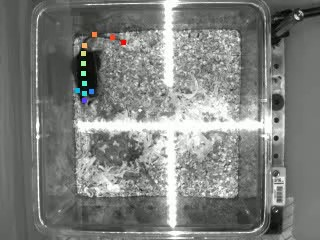
\includegraphics[width=\textwidth, angle=-90]{figures/deeplabcut-top-example-4128-2020-12-02-1-00-37.jpg}
    \caption{}
    \label{fig:deeplabcut-top-example}
  \end{subfigure}
  \begin{subfigure}{0.45\textwidth}
    \centering
    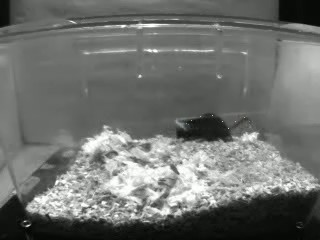
\includegraphics[width=\textwidth]{figures/deeplabcut-lateral-example-4128-2020-12-02-1-00-37.jpg}
    \caption{}
    \label{fig:deeplabcut-lateral-example}
  \end{subfigure}
  \begin{subfigure}{0.45\textwidth}
    \centering
    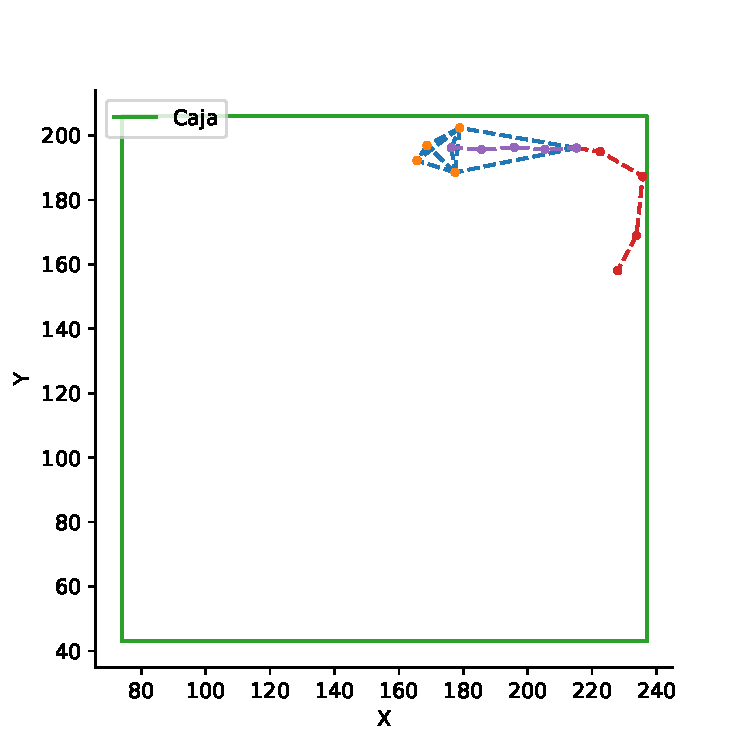
\includegraphics[width=\textwidth]{figures/triangulation-top-4128-2020-12-02.pdf}
    \caption{}
    \label{fig:triangulation-top}
  \end{subfigure}
  \begin{subfigure}{0.45\textwidth}
    \centering
    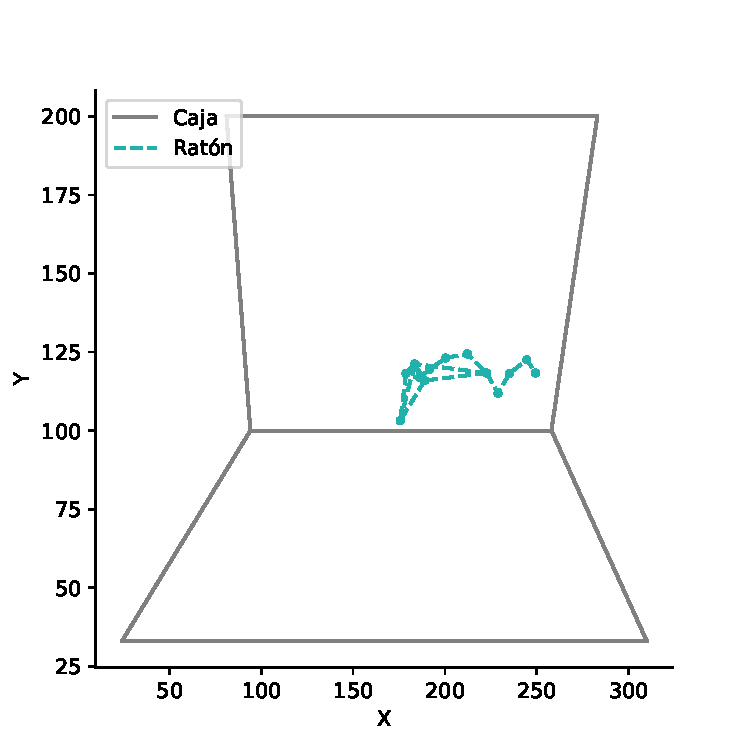
\includegraphics[width=\textwidth]{figures/triangulation-lateral-4128-2020-12-02.pdf}
    \caption{}
    \label{fig:triangulation-lateral}
  \end{subfigure}
  \caption[Salida de DeepLabCut.]
  {Salida de DeepLabCut del animal 4128 el 02-12-2020, 1:00:37. \ref{fig:deeplabcut-top-example} Video de la vista cenital de la caja. Los puntos sobre el animal son los dibujados por DeepLabCut para rastrear las partes del animal. \ref{fig:deeplabcut-lateral-example} Video de la vista lateral de la caja. \ref{fig:triangulation-top} En azul, la triangulación formada por los puntos obtenidos por DeepLabCut de la vista cenital. Cinco puntos para la cabeza, cuatro para la espalda y otros cuatro para la cola. En gris, las dimensiones de la base de la caja, obtenidas midiendo las distancias en píxeles sobre un fotograma de video. \ref{fig:triangulation-lateral} Análogo a la vista cenital, desde la vista lateral. En gris, la altura mínima del suelo de la caja y su pared trasera.}

  \label{fig:deeplabcut-outputexamples}
\end{figure}

\subsection{DeepLabCut}\label{sec:DeepLabCut}
DeepLabCut es una red convolucional profunda que combina redes residuales pre entrenadas con capas deconvolucionales. Una red residual es aquella que concatena cientos de capas convolucionales con capas deconvolucionales que amplían la información visual para producir densidades de probabilidad espaciales. Esto hace que ajustar DeepLabCut para realizar una tarea concreta conlleve únicamente entrenar una red utilizando pocos datos de entrenamiento para obtener un listado de coordenadas de los puntos deseados acompañadas de la verosimilitud de cada uno de los puntos predichos. Las capas deconvolucionales están pre entrenadas con la base de datos de ImageNet \cite{image-net}, una base de datos de imágenes organizadas en conjuntos de sinónimos cognitivos, cada uno agrupando un concepto diferente. El objetivo de ImageNet es proporcionar una buena base de entrenamiento para investigaciones de todo tipo, como por ejemplo la de DeepLabCut. La Figura \ref{fig:diagram-dlc} muestra un esquema de la estructura de la red.

\begin{figure}[h]
  \centering
  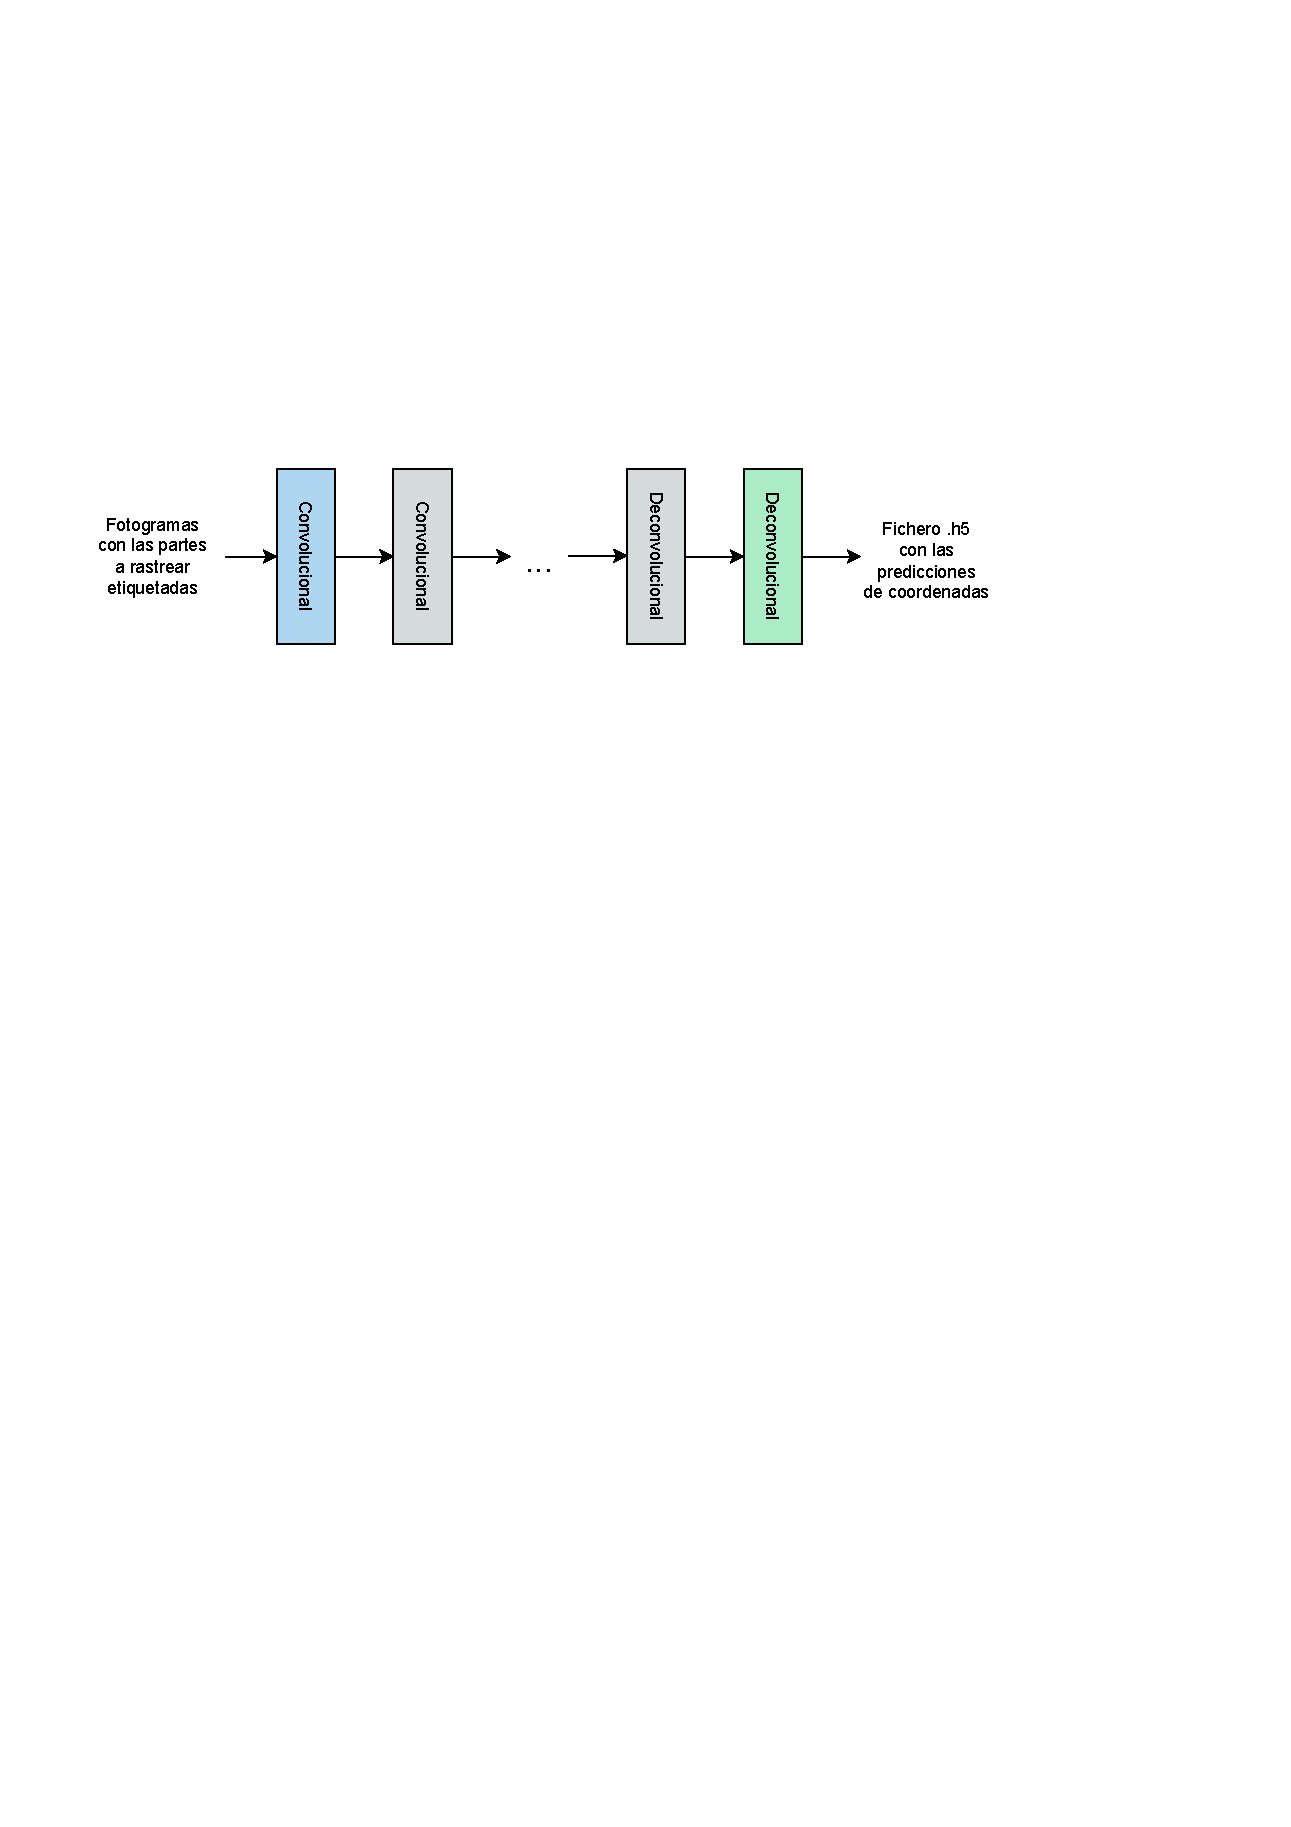
\includegraphics[width=0.9\textwidth]{figures/diagram-dlc.pdf}
  \caption{Diagrama simplificado de la red utilizada por DeepLabCut. La red recibe como entrada los datos de los fotogramas con las partes etiquetadas y los procesa por múltiples capas convolucionales pre entrenadas con ImageNet. Finalmente, las salidas de esas capas pasan por capas deconvolucionales para obtener el fichero con las predicciones de coordenadas.}
  \label{fig:diagram-dlc}
\end{figure}

En el código \ref{code:dcl-dataset} podemos observar como hemos inicializado nuestros conjuntos de datos de entrenamiento para procesar los vídeos de las sesiones. Hemos realizado este proceso para los vídeos cenitales y laterales independientemente, indicando para cada uno de ellos los puntos que queremos rastrear en el fichero de configuración de \texttt{path\_config\_file}. Hemos utilizado también la red residual de 50 capas \texttt{resnet\_50} pre-entrenada por DeepLabCut y seleccionado el método de aumentación de los datos de las capas deconvolucionales \texttt{imgaug}.

\begin{mypython}[caption={Crear datos de entrenamiento de DeepLabCut.}, label={code:dcl-dataset}]
import deeplabcut

deeplabcut.create_training_dataset(path_config_file, 
                                   net_type='resnet_50',
                                   augmenter_type='imgaug')
\end{mypython}

Tras crear los datos de entrenamiento, en el laboratorio se habían etiquetado manualmente 10 fotogramas por sesión, los cuales hemos utilizado en el código \ref{code:dcl-train} para entrenar la red.

\begin{mypython}[caption={Entrenar la red de DeepLabCut.}, label={code:dcl-train}]
deeplabcut.train_network(path_config_file,
                         shuffle=1,
                         trainingsetindex=0,
                         max_snapshots_to_keep=5,
                         displayiters=10,
                         saveiters=250,
                         maxiters=1000,
                         allow_growth=False,
                         autotune=False,
                         keepdeconvweights=True)
\end{mypython}

Tras entrenar la red la evaluamos para verificar que tenemos un error aceptable con el Código \ref{code:dcl-eval}.

\begin{mypython}[caption={Evaluar la red de DeepLabCut.}, label={code:dcl-eval}]
deeplabcut.evaluate_network(path_config_file)
\end{mypython}

Tras entrenar la red, analizamos los vídeos con \texttt{deeplabcut.analyze\_vídeos} obteniendo un fichero \texttt{h5} para cada una de las sesiónes con las cordenadas de todos los puntos rastreados y la verosimilitud de cada uno de los puntos. En la Tabla \ref{tab:df-example} mostramos un fragmento de uno de los ficheros cargado a memoria en un \texttt{DataFrame} para su posterior preprocesado y análisis. Cada uno de los ficheros contiene los datos de 13 partes del animal rastreadas en cada uno de los fotogramas. Las 13 partes se han denominado \texttt{Nose}, \texttt{Head}, \texttt{Neck}, \texttt{Leftear}, \texttt{Rightear}, \texttt{Back\{1-4\}}, \texttt{Tail\{1-4\}}. Por cada una de las partes, DeepLabCut nos proporciona su predición para las coordenadas $ x $ e $ y $ y la verosimilitud de dicha predicción.

Finalmente, utilizando la función \texttt{deeplabcut.create\_labeled\_video} hemos creado dos vídeos de muestra con los puntos rastreados dibujados sobre cada uno de los fotogramas del video como se puede observar en la Figura \ref{fig:deeplabcut-outputexamples}.
% Dataframe example
\begin{table}[h]
  \centering
  \begin{tabular}{|c|c|c|c|c|c|c|}
  \hline
    & Nosex & Nosey & Noselikelihood & Headx & Heady & ... \\
  \hline
  0 & 136.165344 & 177.722496 & 0.000084 & 129.790253 & 174.772552 & ... \\
  1 & 162.032005 & 201.444756 & 0.942181 & 168.152061 & 202.420639 & ... \\
  2 & 156.297043 & 200.326378 & 0.000073 & 162.436028 & 203.156837 & ... \\
  3 & 155.370415 & 199.043297 & 0.000277 & 159.507599 & 200.199928 & ... \\
  4 & 149.272644 & 197.677170 & 0.000045 & 155.493912 & 198.814835 & ... \\
  ... & ... & ... & ... & ... & ... & ... \\
  \hline
  \end{tabular}
  \caption[Datos de DeepLabCut]{Extracto del \texttt{DataFrame} de Pandas de los datos sin procesar de DeepLabCut. Para cada punto rastreado, y para cada fotograma del video, se computa la predicción de la coordenada $x$ y de la coordenada $y$ y se da la verosimilitud de dicha predicción.}
  \label{tab:df-example}
\end{table}

\subsection{Filtrado e interpolación}
Una vez hemos pasado todos los vídeos por DeepLabCut, tenemos dos ficheros de datos para cada uno de las sesiones, uno para las coordenadas de los puntos de la vista cenital y otro para las coordenadas de los puntos de la vista lateral. Al cargar los ficheros a memoria como \texttt{DataFrames} de \texttt{pandas}, observamos que no todos ellos tienen la misma duración, por lo que los homogeneizamos todos eliminando los datos de los últimos fotogramas, consiguiendo que cada \texttt{DataFrame} tenga un tamaño de 6000 filas, lo que equivale a 6000 fotogramas o 5 minutos de video. Además, eliminamos los datos de 4 vídeos que no llegan a esa duración, ya que son vídeos con problemas que entorpecerían el análisis.

Por cada par de coordenadas de cada parte del animal en cada fotograma, DeepLabCut estima la precisión de su predicción y asocia un valor de verosimilitud del par. Antes de trabajar con la salida de DeepLabCut filtramos todos los pares de coordenadas para quedarnos solo con aquellos que tienen una verosimilitud de más de 0,95. Tras el filtrado, interpolamos linealmente las coordenadas eliminadas basándonos en las predicciones de la misma parte más próximas en tiempo con verosimilitud suficiente. En la Figura \ref{fig:interpolated-trayectories} se observa la evolución de los datos de las trayectorias a lo largo del proceso de filtrado e interpolación.

Finalmente, eliminamos los datos de 2 vídeos más, ya que tras el preprocesado seguían teniendo valores nulos debido a que DeepLabCut no ha podido identificar varios de los puntos a rastrear en ninguno de los fotogramas de los vídeos. 

% Trayectory prerpocessing
\begin{figure}[p]
  \centering
  \begin{subfigure}{0.38\textwidth}
    \centering
    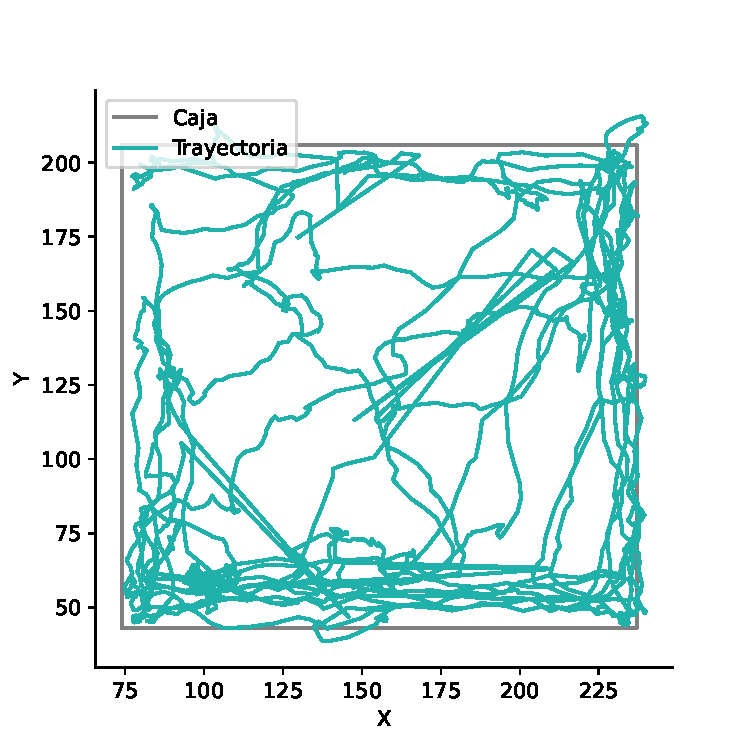
\includegraphics[width=\textwidth]{figures/raw-trayectory-top-4128-2020-12-02.pdf}
    \caption{}
    \label{fig:raw-top}
  \end{subfigure}
  \begin{subfigure}{0.38\textwidth}
    \centering
    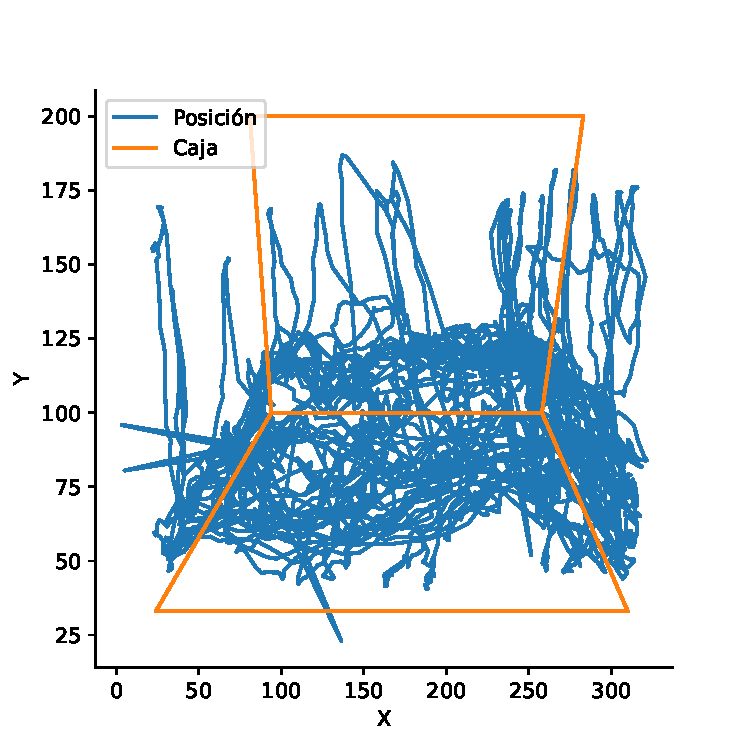
\includegraphics[width=\textwidth]{figures/raw-trayectory-lateral-4128-2020-12-02.pdf}
    \caption{}
    \label{fig:raw-lat}
  \end{subfigure}
  \begin{subfigure}{0.38\textwidth}
    \centering
    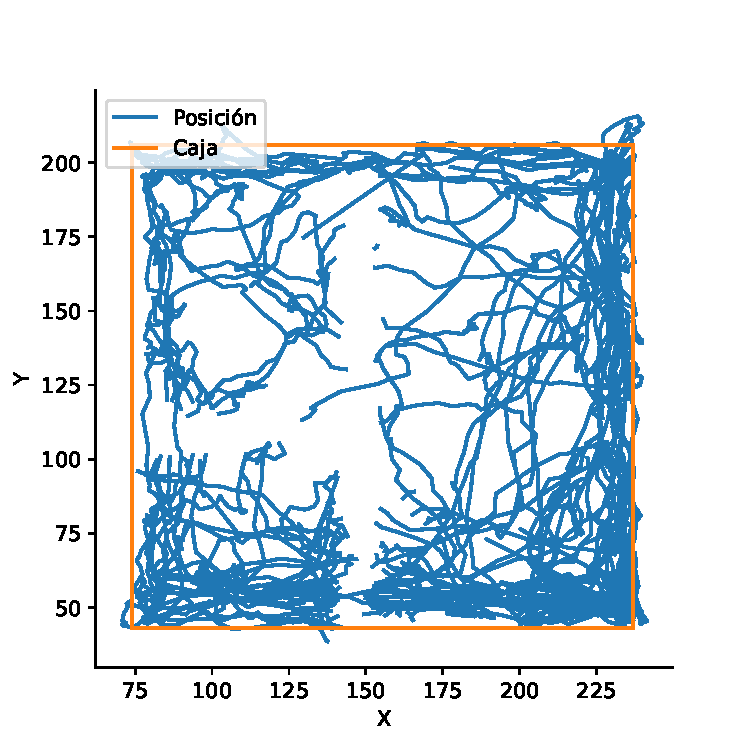
\includegraphics[width=\textwidth]{figures/filtered-trayectory-top-4128-2020-12-02.pdf}
    \caption{}
    \label{fig:filter-top}
  \end{subfigure}
  \begin{subfigure}{0.38\textwidth}
    \centering
    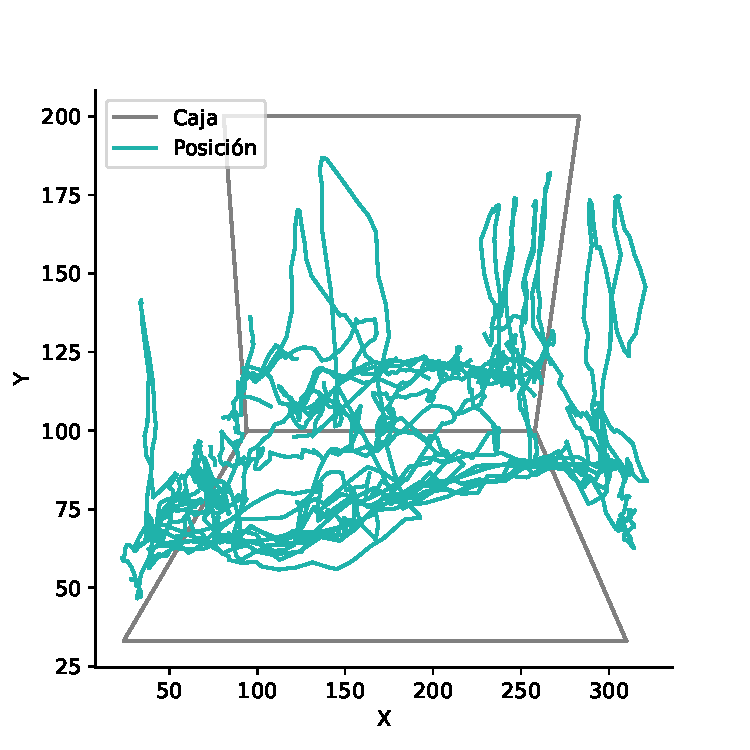
\includegraphics[width=\textwidth]{figures/filtered-trayectory-lateral-4128-2020-12-02.pdf}
    \caption{}
    \label{fig:filter-lat}
  \end{subfigure}
  \begin{subfigure}{0.38\textwidth}
    \centering
    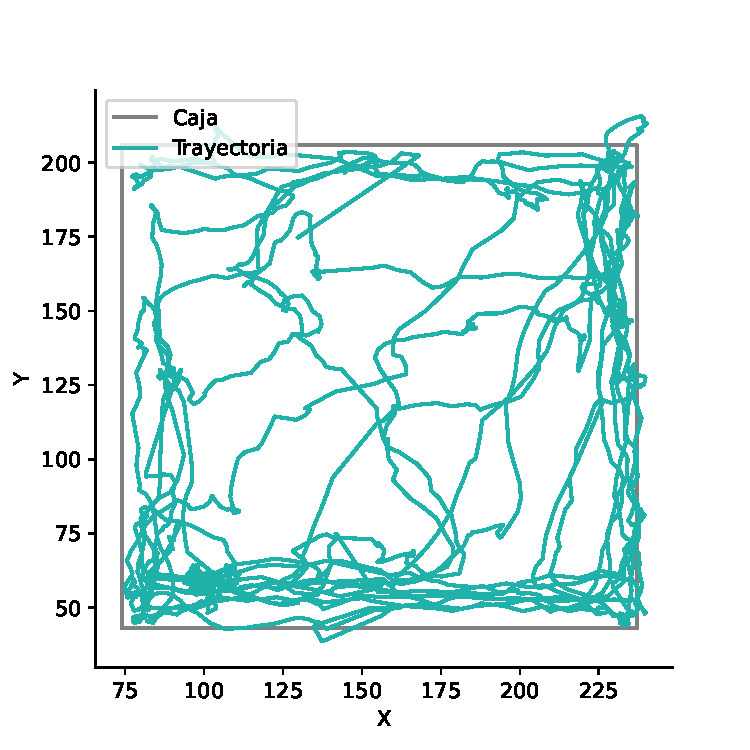
\includegraphics[width=\textwidth]{figures/interpolated-trayectory-top-4128-2020-12-02.pdf}
    \caption{}
    \label{fig:inter-top}
  \end{subfigure}
  \begin{subfigure}{0.38\textwidth}
    \centering
    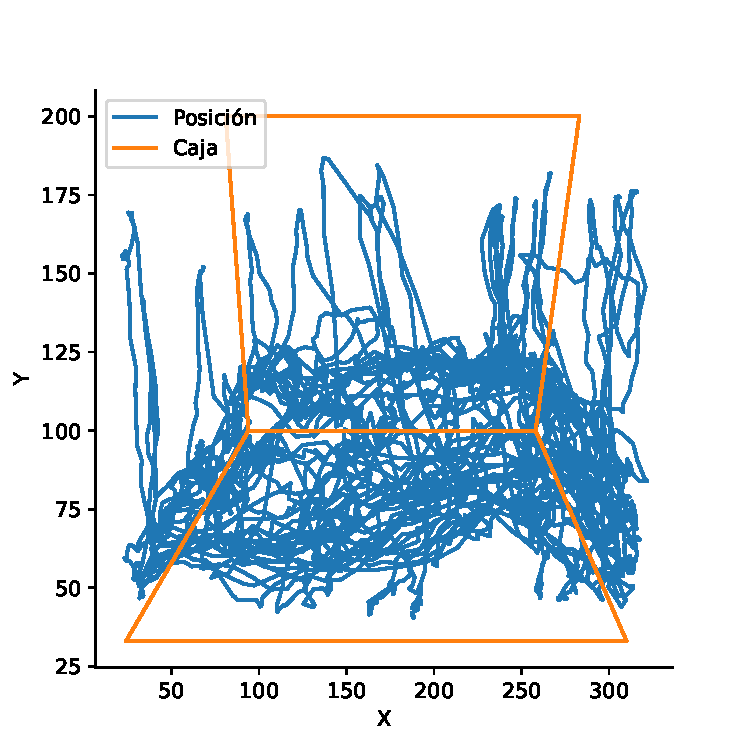
\includegraphics[width=\textwidth]{figures/interpolated-trayectory-lateral-4128-2020-12-02.pdf}
    \caption{}
    \label{fig:inter-lat}
  \end{subfigure}
  \caption[Trayectorias durante el preprocesamiento.]{Vistas cenital y lateral de trayectorias de un punto de la cabeza del animal 4128. Datos correspondientes a los dos primeros minutos de la sesión del 2020-12-02. \ref{fig:raw-top}, \ref{fig:raw-lat}: Vista cenital de los datos antes del preprocesado. En gris se ha dibujado las dimensiones de la caja y en color la trayectoria del punto \texttt{Head}. \ref{fig:inter-top}, \ref{fig:inter-lat}: Vistas cenital y lateral de los datos una vez filtrados los valores de baja verosimilitud. \ref{fig:inter-top}, \ref{fig:inter-lat}: Vistas cenital y lateral de los datos filtrados con los valores nulos interpolados. }
  \label{fig:interpolated-trayectories}
\end{figure}

\section{Análisis de datos} \label{sec:analisis}
En esta sección desarrollamos los diferentes métodos que hemos utilizado en nuestro análisis de los datos, junto con los resultados que hemos ido obteniendo. Primero explicamos los diferentes cómputos manuales que hemos realizado con nuestros datos para identificar ciertos comportamientos y posteriormente explicamos los algoritmos de aprendizaje automático que hemos utilizado para realizar distintas clasificaciones. Para realizar cada uno de los métodos, partimos de los datos de 81 sesiones de video preproesadas. Cada una de las sesiones cuenta con 6000 filas, una por fotograma, y 52 coordenadas, coordenadas $ x $ e $ y $ por cada una de las 13 partes rastreadas por cada una de las dos vistas, cenital y lateral.

\subsection{Clasificación manual de comportamientos}
Gracias a los datos de DeepLabCut podemos tratar de identificar ciertos comportamientos de forma manual, especificando ciertos umbrales para extraer los comportamientos deseados. A modo de ejemplo, hemos calculado cuando el punto de la cabeza en la vista cenital, \texttt{head}, se salía durante un intervalo de cinco fotogramas fuera de los límites establecidos de la caja. Así, como se observa en la Figura \ref{fig:rearing}, hemos identificado los intervalos de tiempo de cada sesión en los cuales el animal se alza sobre sus extremidades traseras apoyándose en la pared de la caja.

% Rearing frames
\begin{figure}[h]
  \centering
  \begin{subfigure}{\textwidth}
    \centering
    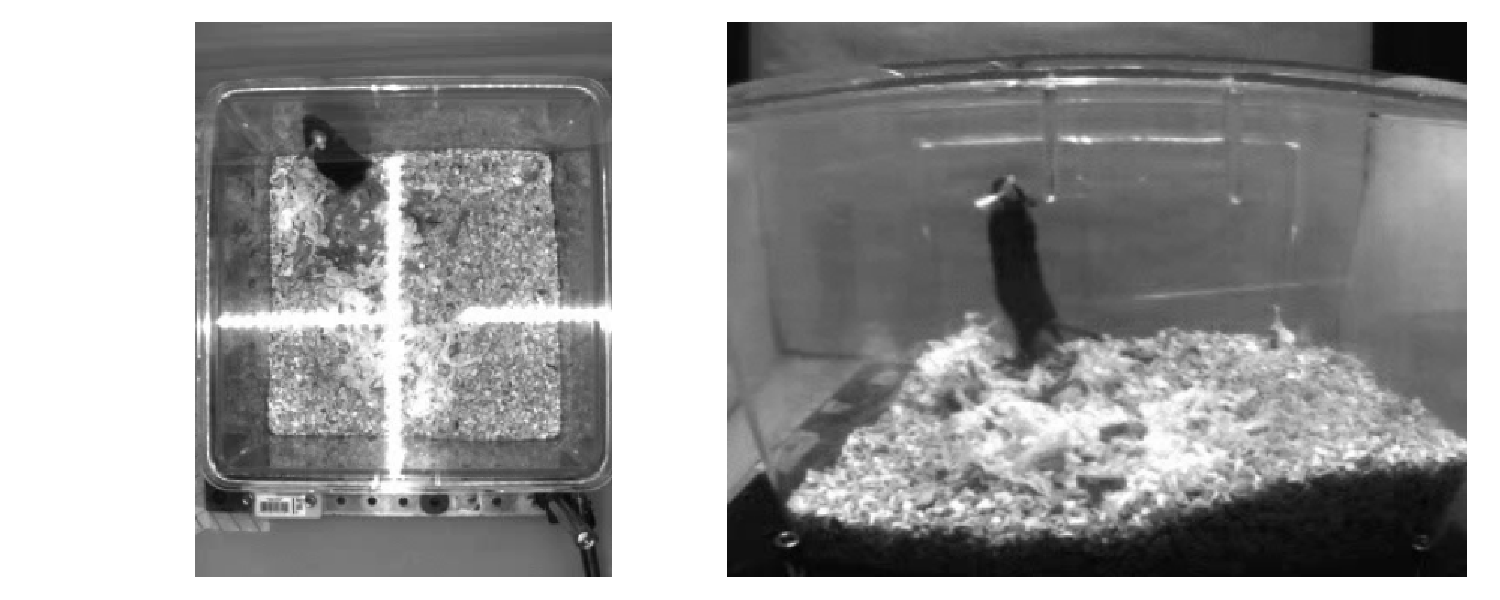
\includegraphics[trim={2cm 0 0 0}, width=0.9\textwidth]{figures/rearing-4128-2020-12-02-0 03.05.pdf}
  \end{subfigure}
  \begin{subfigure}{\textwidth}
    \centering
    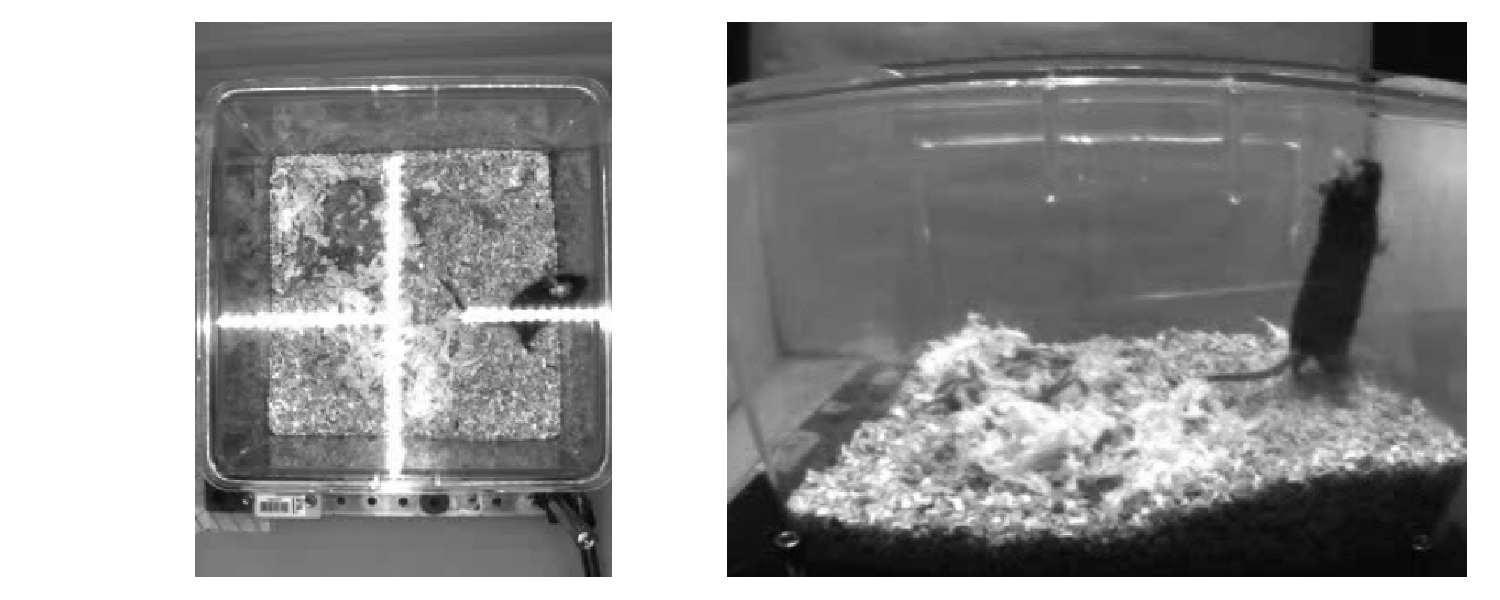
\includegraphics[trim={2cm 0 0 0}, width=0.9\textwidth]{figures/rearing-4128-2020-12-02-0 19.43.pdf}
  \end{subfigure}
  \caption[Fotogramas del animal alzándose.]{Fotogramas de los dos primeros intervalos en los que el animal 4128 se alza en la sesión del 2020-12-02. Los fotogramas superiores corresponden a la vista cenital y lateral del segundo 3,05. Los fotogramas inferiores corresponden a las mismas vistas del segundo 19,43.}
  \label{fig:rearing}
\end{figure}

De la misma forma, podemos calcular en que intervalos la media de los puntos de la espalda tienen una velocidad mayor de tres píxeles por segundo para identificar cuando el animal se está moviendo como se puede ver en la Figura \ref{fig:speed}, o calcular el ángulo formado entre un vector de los puntos de la cabeza del animal y otro de los puntos de la espalda, para determinar si el animal está girado hacia algún lado, visualizado en la Figura \ref{fig:angles}.

% Speed
\begin{figure}[h]
  \centering
  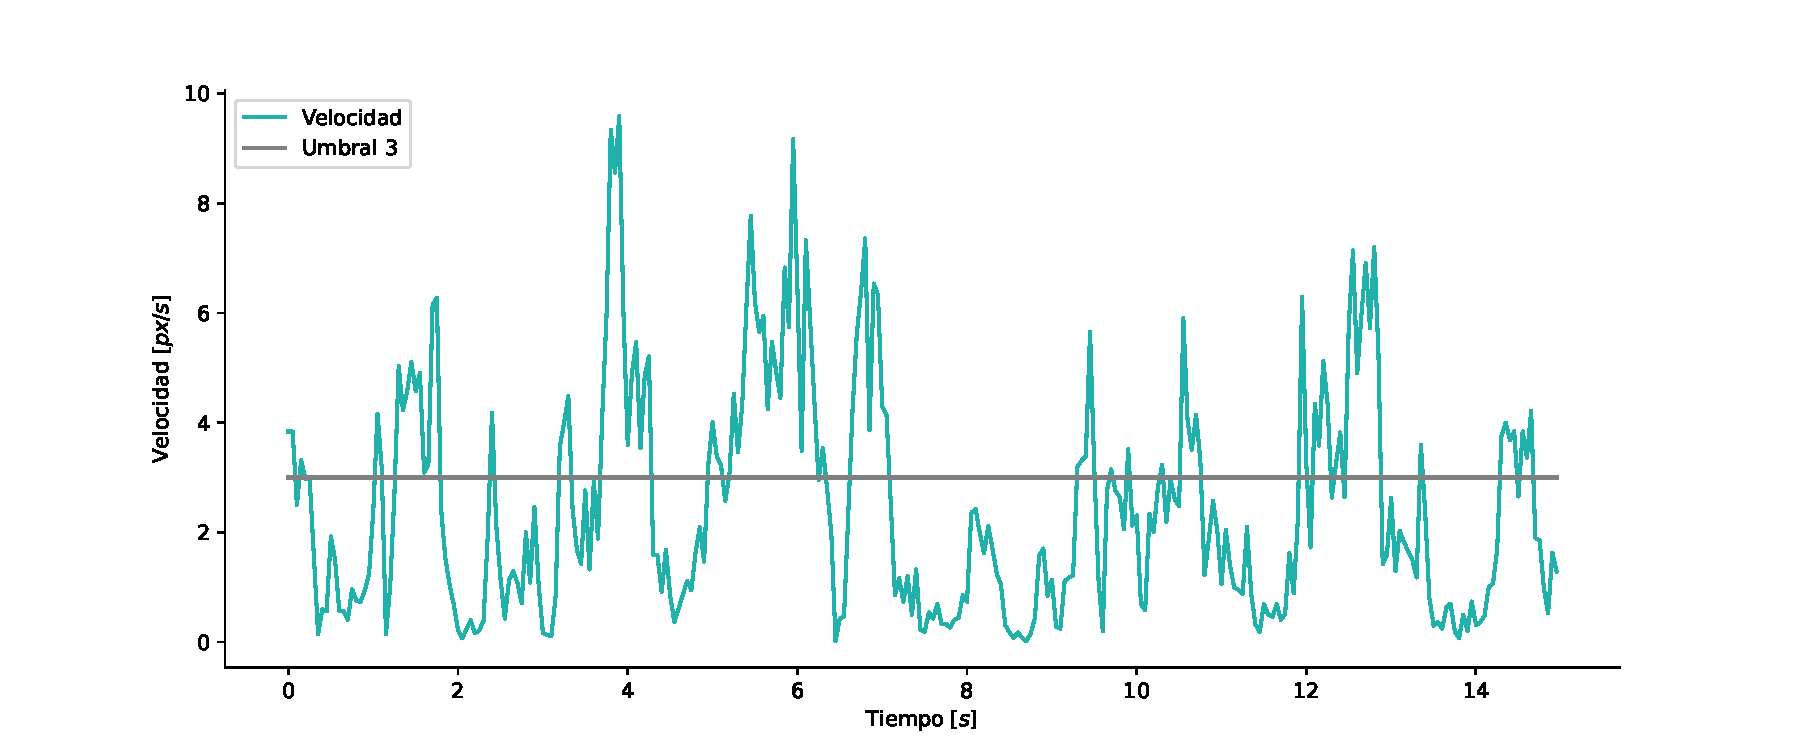
\includegraphics[width=\textwidth]{figures/speed-4128-2020-12-02-threshold-3-15s.pdf}
  \caption[Velocidad del animal.]{Gráfico de la velocidad del animal 4128, durante los primeros 15 segundos de la sesión del 2020-12-02. En color, los datos obtenidos derivando la trayectoria de la media de los puntos de la espalda del animal: \texttt{Neck}, \texttt{Back\_1}, \texttt{Back\_2}, \texttt{Back\_3} y \texttt{Back\_4}. En gris, el umbral arbitrario de 3 píxeles por segundo, para diferenciar cuando el animal está desplazándose y cuando no.}
  \label{fig:speed}
\end{figure}

% Angles
\begin{figure}[h]
  \centering
  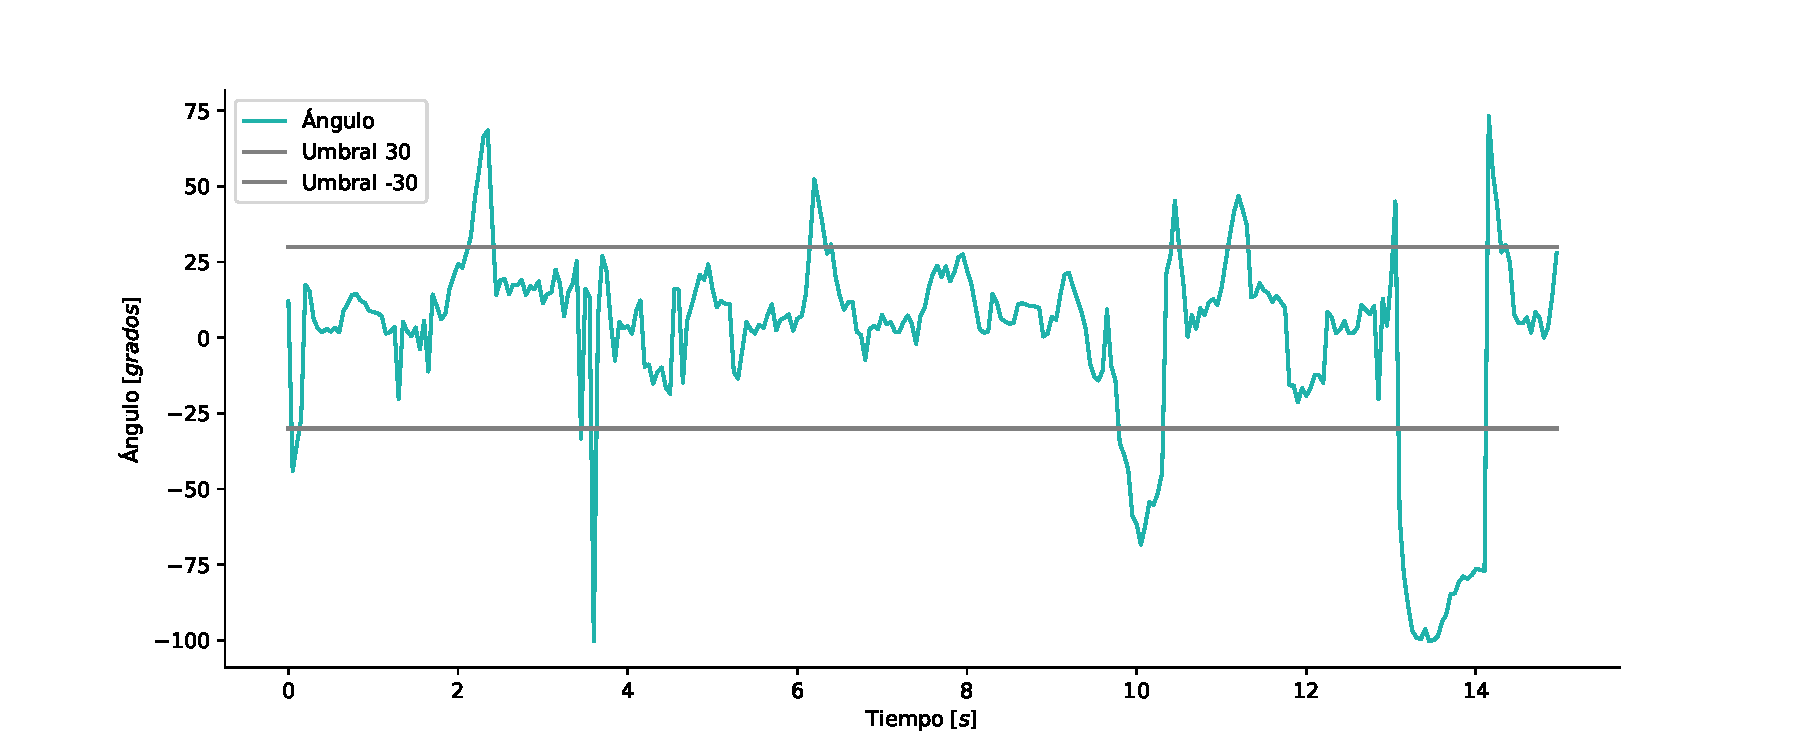
\includegraphics[width=\textwidth]{figures/angles-4128-2020-12-02-threshold-30-15s.pdf}
  \caption[Ángulos del animal.]{Gráfico de los ángulos del animal 4128, durante los primeros 15 segundos de la sesión del 2020-12-02. En color, el ángulo formado por el vector de los puntos de la cabeza con el vector de los puntos de la espalda. En gris, los umbrales de 30° y -30° para determinar si el animal está recto, o tiene el cuerpo girado hacia la izquierda o derecha respectivamente,}
  \label{fig:angles}
\end{figure}

Estos métodos de extracción de comportamientos funcionan para este caso particular, pero al depender de funciones hechas específicamente para estos datos, sería complejo exportarlo a otros escenarios. DeepLabCut ayuda en ese aspecto, ya que no calculamos propiedades sobre los vídeos en sí, sino sobre un conjunto de coordenadas de posiciones de partes del animal. De esta forma, si se tratase de analizar vídeos de animales grabados en otras cajas o realizando alguna tarea, podríamos computar de forma sencilla estas propiedades ajustando los parámetros necesarios.

Sin embargo, para el cómputo manual de estas propiedades se han puesto umbrales arbitrarios para definir el estado del animal. Un umbral de 3 píxeles por segundo sobre la media de los puntos de la espalda para determinar cuando el animal se está desplazando, un umbral de ±30° para determinar si el animal está girando o no, o un umbral de 5 fotogramas fuera de las dimensiones de la caja para determinar si el animal se está alzando sobre una pared. Los umbrales son necesarios si consideramos necesario discretizar estas variables continuas en comportamientos cualitativos, pero están a su vez sesgados por el juicio del experimentador, ya que una varianza en la magnitud de los umbrales o en el conjunto de puntos utilizados para calcularlos puede resultar en una discrepancia de la clasificación obtenida.

La clasificación manual hace que sea complejo determinar también cuando el animal realiza algún comportamiento más complejo que los vistos hasta ahora, ya que si no sabemos de antemano la relación entre las coordenadas de las partes del animal y el comportamiento, no podremos identificarlo. De la misma forma, al no conocer de antemano la relación entre los diferentes comportamientos y el tipo de tratamiento dado a los animales, con estas clasificaciones no se podrán diferenciar animales tratados con anticuerpos de NMDA de animales control.

Esto motiva las siguientes secciones en las cuales hemos utilizado diversos métodos de aprendizaje automático para tratar de conseguir clasificaciones sin depender de sesgos preestablecidos.

\subsection{Agrupaciones no supervisadas}
Para tratar de automatizar el proceso de clasificación, sin depender de cualidades computadas \textit{ad hoc} para este conjunto de datos, hemos aplicado los algoritmos vistos en la sección \ref{sec:unsupervised} sobre los datos de las trayectorias preprocesados según hemos visto en la sección \ref{sec:preprocesado}.

Para clasificar los comportamientos de un animal en cada sesión no contamos ejemplos de comportamientos identificados y previamente clasificados por lo que no podemos hacer uso de métodos de aprendizaje automático supervisados. Además, si no queremos introducir un sesgo en la clasificación, tampoco sabemos de antemano en cuantos grupos de comportamiento similares podremos agrupar los diferentes fragmentos de cada sesión de video. Por ello hemos utilizado un algoritmo de propagación de afinidad, basándonos en el trabajo realizado por A. Klaus et al. \cite{neuron}. Dicho algoritmo nos permite agrupar fragmentos de comportamiento función de su afinidad. Hemos dividido los vídeos de las sesiones en intervalos de 5 segundos e introducido los datos de las coordenadas de todos los puntos de las vistas cenital y lateral para todos los puntos de cada fotograma de los intervalos. En la Figura \ref{fig:unsupervied-behav} se muestra la agrupación obtenida para la sesión de uno de los animales, consiguiendo agrupar los distintos intervalos en 7 grupos de comportamiento.

% Behav aff
\begin{figure}[h]
  \centering
  \begin{subfigure}{0.45\textwidth}
    \centering
    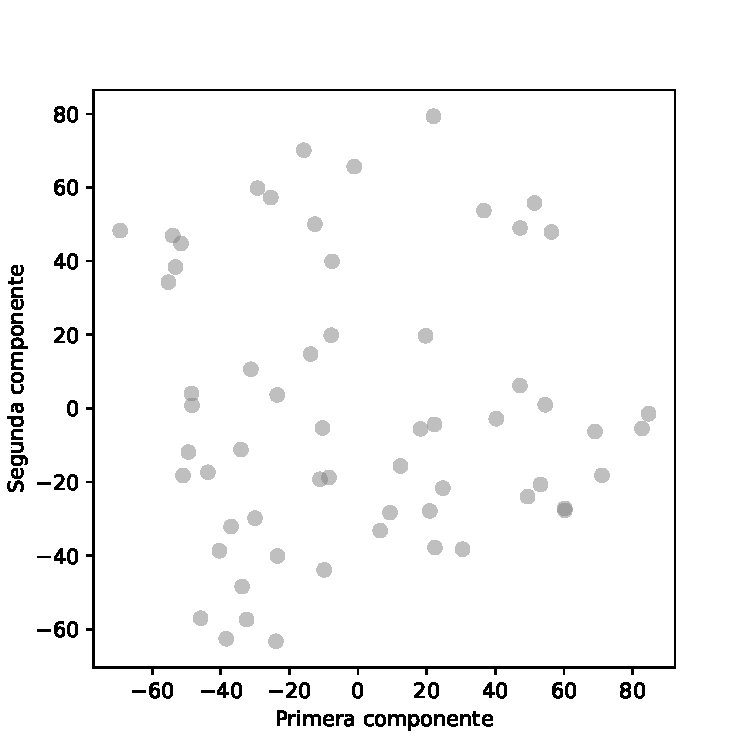
\includegraphics[width=\textwidth]{figures/behav-pca-4128-202012-02.pdf}
    \caption{}
    \label{fig:behav-pca}
  \end{subfigure}
  \begin{subfigure}{0.45\textwidth}
    \centering
    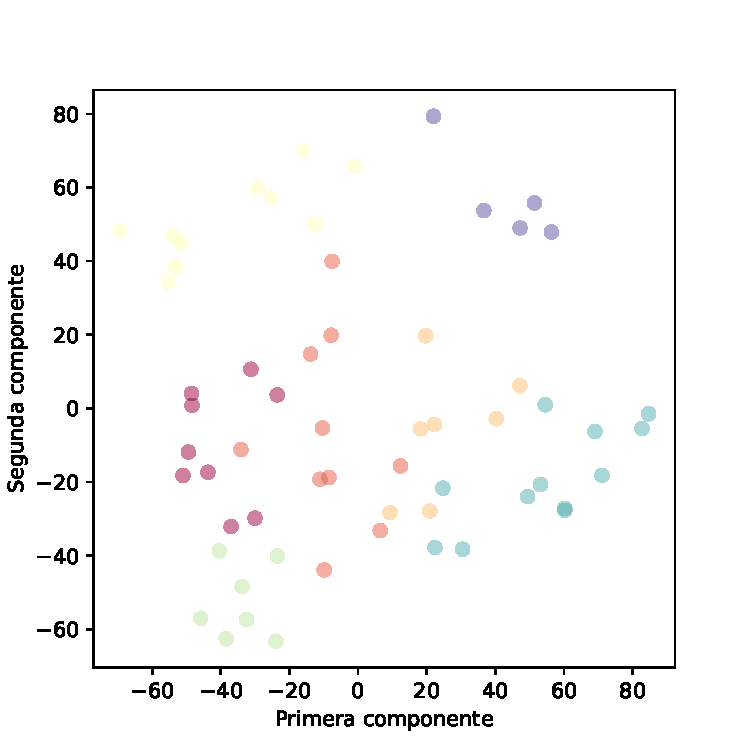
\includegraphics[width=\textwidth]{figures/behav-aff-4128-202012-02.pdf}
    \caption{}
    \label{fig:behav-aff}
  \end{subfigure}
  \caption[Clasificación no supervisada de comportamiento.]{Clasificación de comportamiento mediante el algoritmo de propagación de afinidad sobre intervalos de la sesión del animal 4128 el 2020-12-02. \ref{fig:behav-pca}: Distribución de los puntos de un PCA sobre una subdivisión de la sesión en 60 intervalos. Cada punto representa un intervalo de 5 segundos, 100 fotogramas, de la sesión de video. Cada punto original cuenta con 56 dimensiones, correspondientes a las coordenadas $ x $ e $ y $ de los 13 puntos extraídos por DeepLabCut tanto para la vista cenital como la vista lateral. Todos los puntos se han normalizado para tener media 0 y desviación 1 antes de realizar el PCA. Tras el PCA, y únicamente para su representación gráfica, se conservan las dos primeras componentes principales de cada punto. \ref{fig:behav-aff}: Misma representación de los 60 intervalos que en \ref{fig:behav-pca}, pero los puntos han sido coloreados según el número de grupo asignado por el algoritmo de propagación de afinidad. El algoritmo se ha realizado sobre los puntos de los intervalos normalizados, manteniendo las 56 dimensiones originales y utilizando la norma euclídea como medida de afinidad.}
  \label{fig:unsupervied-behav}
\end{figure}

No podemos usar el algoritmo de propagación de afinidad para diferenciar el tipo de tratamiento de cada una de las sesiones, ya que no es posible garantizar que vaya a generar dos únicas clases. Por ello, hemos utilizado los otros dos algoritmos explicados en la sección \ref{sec:unsupervised}: la agrupación por k-medias y la agrupación aglomerativa, ambos utilizados en estudios similares \cite{frontiers}. Para ambos casos hemos tomado los datos de todas las sesiones y tras aplicarles el algoritmo hemos mostrado los resultados en la Figura \ref{fig:unsupervied-treatment}. Con ninguno de los dos algoritmos hemos conseguido resultados mejores que los que obtendríamos haciendo asignaciones aleatorias de las clases, por lo que no podemos asegurar que exista alguna relación directa entre la posición de los animales y el tipo de tratamiento que se les ha suministrado.

Para conseguir realizar esta clasificación habría que computar otras características manualmente con las que dar más información a los algoritmos, cambiar los puntos rastreados por DeepLabCut para conseguir información sobre otras partes del animal, o tratar de predecir una función desconocida que fuera capaz de agrupar las sesiones correctamente. Como tenemos los datos de todas las sesiones podemos entrenar métodos supervisados, y estamos en las condiciones idóneas para tratar de predecir, en caso de que exista, esa función que relacione las coordenadas de los puntos que hemos rastreado con el tipo de tratamiento de cada sesión.

% Treatment kmean agg
\begin{figure}[p]
  \centering
  \begin{subfigure}{0.45\textwidth}
    \centering
    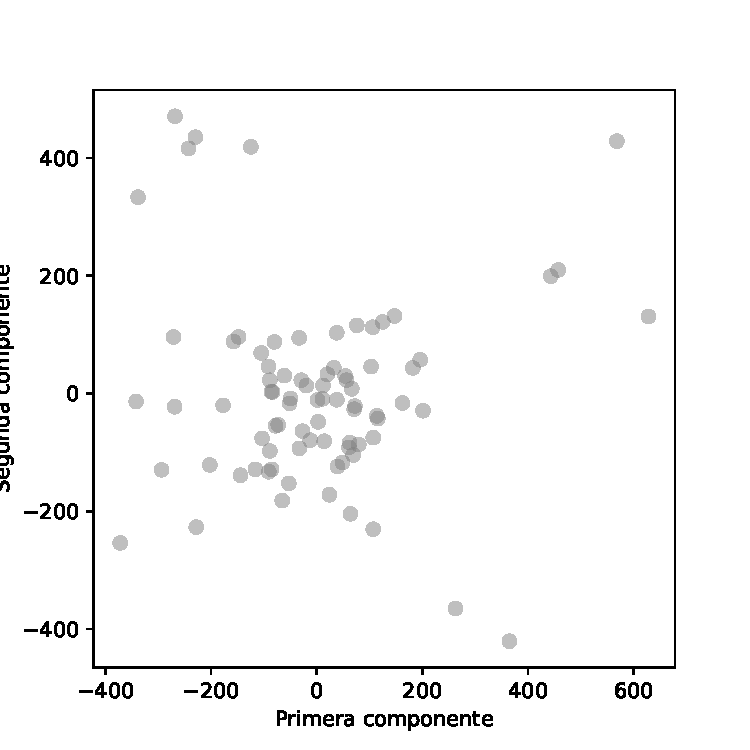
\includegraphics[width=\textwidth]{figures/pca-all-sessions-trayectory.pdf}
    \caption{}
    \label{fig:treat-pca}
  \end{subfigure}
  \begin{subfigure}{0.45\textwidth}
    \centering
    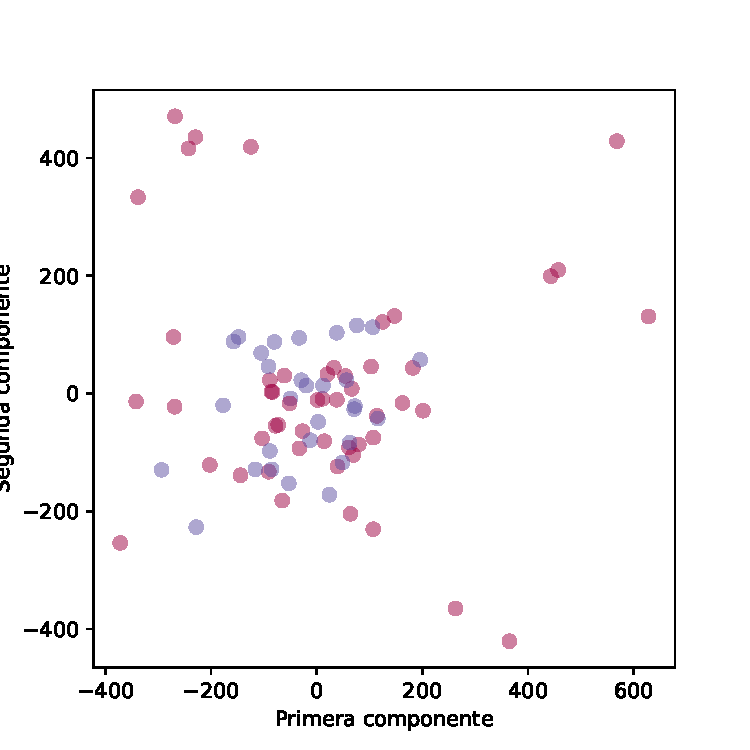
\includegraphics[width=\textwidth]{figures/true_asg-all-sessions-trayectory.pdf}
    \caption{}
    \label{fig:treat-true}
  \end{subfigure}
  \begin{subfigure}{0.45\textwidth}
    \centering
    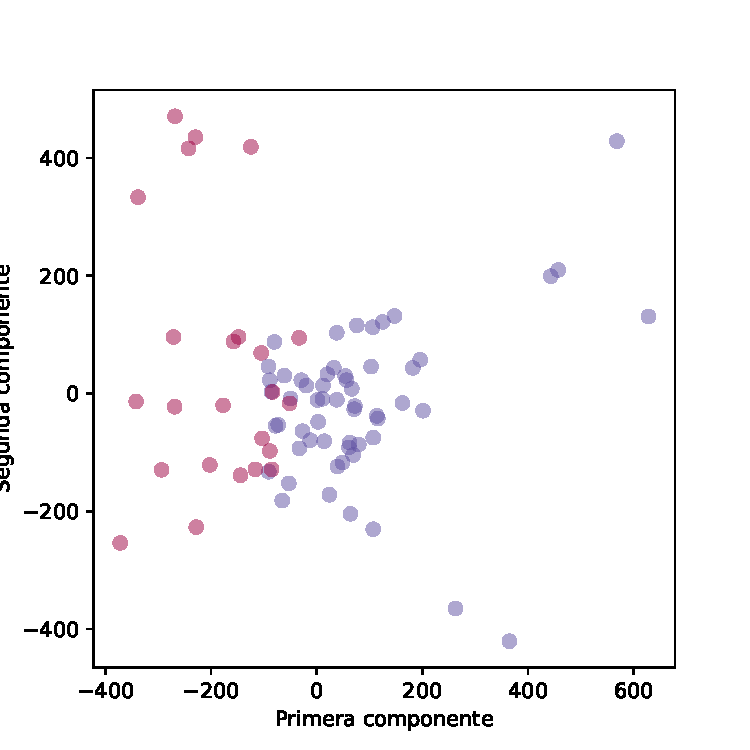
\includegraphics[width=\textwidth]{figures/kmeans_asg-all-sessions-trayectory.pdf}
    \caption{}
    \label{fig:treat-kmean}
  \end{subfigure}
  \begin{subfigure}{0.45\textwidth}
    \centering
    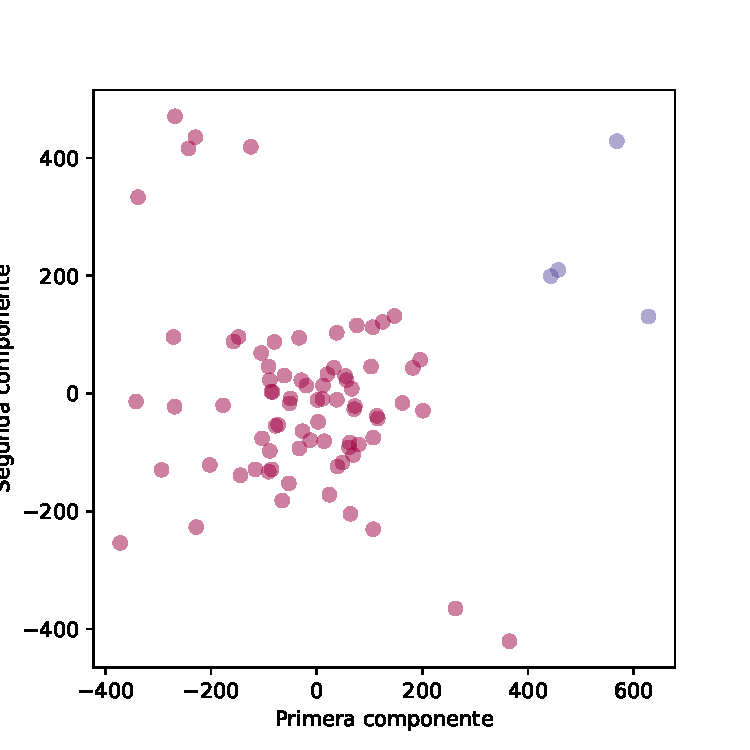
\includegraphics[width=\textwidth]{figures/agg_asg-all-sessions-trayectory.pdf}
    \caption{}
    \label{fig:treat-agg}
  \end{subfigure}
  \caption[Clasificación no supervisada de tratamiento.]{Clasificaciones no supervisadas del tipo de tratamiento. \ref{fig:treat-pca}: Distribución de los puntos de un PCA realizado sobre los datos de las 81 sesiones preprocesados y normalizados. Cada punto tiene una dimensión original de 6000 fotogramas por 52 coordenadas por fotograma, que se han linealizado para tener 312000 dimensiones por punto antes de realizar el PCA. \ref{fig:treat-true}: Asignación real del estado de cada tratamiento para cada sesión. En azul se han marcado las sesiones bajo el efecto de anticuerpos de NMDA y en rosa se han marcado las sesiones en las que no hay efecto, o se ha suministrado un tratamiento placebo. \ref{fig:treat-kmean}: Resultados de una agrupación mediante un algoritmo de k-medias sobre los puntos de las 81 sesiones con todas las dimensiones, mostrado sobre los puntos obtenidos mediante el PCA. Clases agrupadas con una precisión del $ 51,85\% $. \ref{fig:treat-agg} Resultados de una agrupación mediante un algoritmo de agrupación aglomerada sobre los puntos de las 81 sesiones con todas las dimensiones, mostrado sobre los puntos obtenidos mediante el PCA. Clases agrupadas con una precisión del $ 58,02\% $.}
  \label{fig:unsupervied-treatment}
\end{figure}

\subsection{Agrupaciones supervisadas}

Para aproximar una función que relacione las coordenadas de los puntos rastreados por DeepLabCut con el estado de los animales en cada sesión de video, hemos realizado una red neuronal con dos capas convolucionales para relacionar propiedades comunes de fotogramas próximos en el tiempo, y con otras dos capas lineales para asociar las propiedades encontradas con una de las dos clases que queremos diferenciar: animales con tratamiento control o previos al tratamiento con anticuerpos anti NMDA, y animales que están bajo los efectos del tratamiento de anticuerpos anti NMDA.

Las redes convolucionales son usadas generalmente para el tratamiento de imágenes haciendo convoluciones bidimensionales, como por ejemplo en las redes de DeepLabCut. Como nuestros datos tienen una estructura de serie temporal, hemos realizado convoluciones unidimensionales con las capas \texttt{nn.Conv1d} de PyTorch. En datos de imágenes la convolución obtiene propiedades de píxeles próximos, en las series temporales se obtienen propiedades de momentos temporales próximos, fotogramas en nuestro caso.

Para preparar nuestros datos para entrenar y validar nuestra red hemos creado una subclase del tipo \texttt{Dataset} de PyTorch en la cual introducimos los \texttt{DataFrame} con los datos de las sesiones y las etiquetas de cada una de ellas para almacenarlas juntas y tener asociados los datos cada sesión con su etiqueta correspondiente. Podemos ver la implementación de esta clase en el Código \ref{code:dataset}. Al almacenar los datos también los normalizamos con el \texttt{StandardScaler} de Scikit-learn para facilitar la optimización de las funciones de la red. Además, hemos subdividido cada sesión de 5 minutos en fragmentos de un minuto para ampliar la cantidad de nuestros datos de prueba. Esto supone pasar de tener sesiones de 6000 fotogramas a sesiones de 1200, reduciendo a su vez la dimensión de cada uno de los puntos. Por contra, esto supone asumir que el periodo de tiempo de un minuto es suficiente para detectar patrones que puedan indicar el estado del tratamiento de un animal.

% Dataset
\begin{mypython}[float={h}, caption=\texttt{Dataset} de las sesiones, label={code:dataset}]
class SessionDataset(Dataset):
  def __init__(self, dataframes, labels):
    self.data = dataframes
    self.labels = np.array(labels)
    
    # Fit the scaler on the entire dataset
    self.scaler = StandardScaler()
    self.scaler.fit(np.concatenate(self.data))  

  def __len__(self):
    return len(self.data)

  def __getitem__(self, idx):
    # Convert dataframe to numpy array
    data = self.data[idx].values 

    # Normalize the data
    data = self.scaler.transform(data)

    label = self.labels[idx]
    data_tensor = torch.tensor(data, dtype=torch.float)
    return data_tensor.permute(1, 0), label

dataset = SessionDataset(split_dfs,
                         split_animal_info['real-assigment'])
\end{mypython}

En el Código \ref{code:convolutional} podemos ver la implementación en PyTorch de la red que hemos diseñado, y en la Figura \ref{fig:diagram-conv-lab} un esquema con la estructura de la misma. Cuenta con un total de cuatro capas, dos convolucionales y dos lineales. La primera capa convolucional cuenta con una 52 canales de entrada, uno por cada coordenada de un fotograma. Su núcleo de tamaño 20 hace que al recorrer los 1200 fotogramas se asocien como próximos en grupos de 20, buscando estructuras de comportamiento de hasta un segundo. La capa tiene 104 salidas, duplicando el tamaño de los datos antes de introducirlos en la siguiente capa. Hemos utilizado una función de activación \texttt{relu} siguiendo los estándares de la mayoría a de redes de clasificación y hemos reducido la dimensionalidad de los datos en 2 antes de pasar los datos a la siguiente capa mediante la función \texttt{max\_pool\_1d}.

\begin{figure}[h]
  \centering
  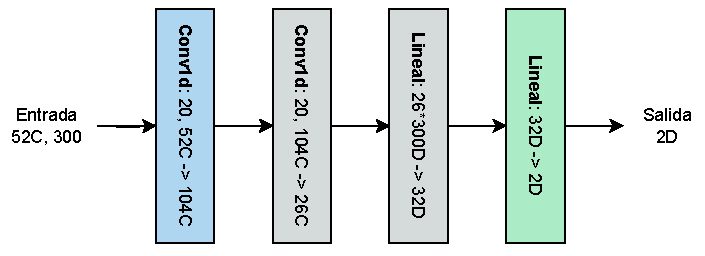
\includegraphics[width=0.9\textwidth]{figures/diagram-conv-lab.pdf}
  \caption{Diagrama de la red utilizada para analizar nuestros datos. La red recibe como entrada datos con 300 instantes temporales de 52 canales cada uno. Estos pasan a la siguiente capa duplicando los canales y a la tercera recudiéndose a 26. En las capas convolucionales, se usa un núcleo de tamaño 20, por lo que cada dato procesado solo tiene encuentra intervalos de 20 fotogramas próximos entre sí.}
  \label{fig:diagram-conv-lab}
\end{figure}

La segunda capa de nuestra red es otra convolucional que ahora reduce el número de canales de 104 a 26 con el mismo núcleo que la capa anterior, y volviendo a usar la misma función de activación y de reducción de dimensionalidad. Tras aplicar estas dos capas convolucionales nos quedan datos de 26 canales respecto a los 52 originales y 300 puntos, respecto a los 1200 con los que empezamos.

Finalmente aplicamos dos capas lineales como en las redes secuenciales tradicionales para transformar la salida de las capas convolucionales primero de 26 * 300 dimensiones a 32, y finalmente de esas 32 a 2 para determinar, para cada minuto de sesión, una de las dos clasificaciones que buscamos.

% Network
\begin{mypython}[float={h}, caption=Red convolucional, label={code:convolutional}]
import torch.nn.functional as F

class TimeSeriesNet(nn.Module):
  def __init__(self):
    super().__init__()
    self.conv1 = nn.Conv1d(in_channels=52, out_channels=104,
                           kernel_size=20, padding=10)
    self.conv2 = nn.Conv1d(in_channels=104, out_channels=26,
                           kernel_size=20, padding=10)
    self.fc1 = nn.Linear(26 * 300, 32)
    self.fc2 = nn.Linear(32, 2)

  def forward(self, x):
    # Input shape: (batch_size, channels, sequence_length)

    # Max pooling with kernel size 2
    out = F.max_pool1d(F.relu(self.conv1(x)), 2)  
    out = F.max_pool1d(F.relu(self.conv2(out)), 2)

    # Flatten for fully connected layer
    out = out.view(out.size(0), -1)  
    out = F.relu(self.fc1(out))
    out = self.fc2(out)
    return out
\end{mypython}

Para entrenar y validar nuestra red, obteniendo una medida estadísticamente robusta de la precisión de la misma, hemos utilizado un método de validación cruzada, separando nuestros datos en cinco grupos aleatorizados con un 20\% de los fragmentos de sesiones cada uno. Así, hemos entrenado cinco modelos de la misma red, cada uno con un 80\% de los datos, dejando en cada caso un 20\% de los datos diferente para realizar la validación. En el Apéndice \ref{apen:salida-conv} hemos trascrito la salida del entrenamiento de los diferentes modelos observando que se obtienen precisiones que oscilan entre el 46 y 71\% de tasa de acierto, con una media final del 58,27\%, un porcentaje no muy superior al de realizar una asignación de clases aleatoria.

Esta baja precisión puede estar causada por diversos factores, entre los cuales pueden estar la poca cantidad de datos de entrenamiento, el uso de una red demasiado genérica y poco adaptada al problema, o la posibilidad de que no exista una relación entre las coordenadas de los puntos rastreados de las partes del animal y el estado del tratamiento del mismo.